\documentclass[a4paper,14pt]{extarticle}
\usepackage{fontspec, unicode-math}
\usepackage[english, russian]{babel}
\setmainfont{Times New Roman}
\setmonofont{CMU Typewriter Text}

\usepackage{enumitem}
\usepackage{alltt}

\usepackage{graphicx}
\usepackage{float}
\usepackage{caption}
\captionsetup[figure]{name={Рисунок}}

% === WIP ===

\usepackage{xcolor}
\newcommand{\todo}[1]{\textbf{\textcolor{red}{#1}}}

% === Formatting ===
% Based on https://github.com/3ap/ifmo-vkr-preamble

\usepackage[top=20mm, bottom=20mm, left=25mm, right=10mm]{geometry}

\usepackage[nodisplayskipstretch]{setspace}
\onehalfspacing

\addto\captionsrussian{
  \renewcommand{\contentsname}{Оглавление}
}

\usepackage{indentfirst}
\setlength{\parindent}{1.25cm}

\usepackage{titlesec}
\titleformat{\section}[block]{\centering\bfseries\large}{\arabic{section}}{1ex}{\MakeUppercase}
\titleformat{\subsection}[block]{\hspace{\parindent}\bfseries\normalsize}{\arabic{section}.\arabic{subsection}}{1ex}{}
\titleformat{\subsubsection}[block]{\hspace{\parindent}\bfseries\normalsize}{\arabic{section}.\arabic{subsection}.\arabic{subsubsection}}{1ex}{}
\titlespacing*{\section}{0pt}{42pt}{42pt}

% Avoid overfull boxes by stretching word spacing
\setlength\emergencystretch{\hsize}

% === Bibliography ===

\usepackage[parentracker=true,
  backend=biber,
  language=russian,
  autolang=other,
  sorting=none,
  citestyle=gost-numeric,
  bibstyle=gost-numeric,
]{biblatex}
\addbibresource{thesis.bib}

\usepackage{xurl}
\usepackage[hidelinks]{hyperref}

% === Commands ===

\newcommand{\topic}[1]{\textbf{#1.}}

\newcommand{\var}[1]{\mathop{\mathit{#1}}}

\newenvironment{ul}{\begin{itemize}[noitemsep,topsep=0em]}{\end{itemize}\vspace{20pt}}

\newenvironment{ol}{\begin{enumerate}[noitemsep,topsep=0em]}{\end{enumerate}\vspace{20pt}}

\newenvironment{inlineul}{\begin{itemize}[noitemsep,topsep=0em]}{\end{itemize}}

\newenvironment{inlineol}{\begin{enumerate}[noitemsep,topsep=0em]}{\end{enumerate}}

% === Body ===

\begin{document}

\tableofcontents
\newpage

\section*{ТЕРМИНЫ И ОПРЕДЕЛЕНИЯ}
\phantomsection\addcontentsline{toc}{section}{ТЕРМИНЫ И ОПРЕДЕЛЕНИЯ}

\textit{Шейдер} — программа, предназначенная для исполнения на графическом процессоре.

\newpage

\section*{ВВЕДЕНИЕ}
\phantomsection\addcontentsline{toc}{section}{ВВЕДЕНИЕ}

\topic{Актуальность темы исследования} Графические процессоры широко используются
для математических расчетов, в частности, в машинном обучении. Для достижения оптимальной
утилизации аппаратных ресурсов алгоритмы реализуются при помощи ассемблера. Отсутствие
средств верификации ассемблерных программ для ГП затрудняет разработку и
может привести к некорректным результатам во время исполнения.

Особый интерес представляют графические процессоры AMD, которые предоставляют разработчику
на ассемблере доступ к аппаратному набору команд. В связи с особенностями аппаратной
реализации от программиста требуется ручное разрешение зависимостей по данным
путем вставки специальных инструкций.

Ошибки в разрешении зависимостей могут быть обнаружены методами статического анализа
еще на этапе разработки программы. Задача осложняется тем, что при разработке
на ассемблере используются различные препроцессоры и трансляторы кода. В работе
предлагается анализ исполняемых файлов, который позволяет работать с единым
представлением программы, которое не зависит от инструментов, используемых при разработки.\\

\topic{Степень теоретической разработанности темы} Статический анализ исполняемых файлов
широко рассмотрен в работах, посвященных информационной безопасности, а именно:
дизассемблированию обфусцированного кода и обнаружению вирусов,
проверке недоверенного кода в плагинах на некорректный доступ к памяти и т.д.\cite{static-analysis-binary}

Существующие средства статического анализа для графических процессоров работают с
высокоуровневыми языками (CUDA, OpenCL) и направлены на обнаружение состояний
гонки (\textit{data races}), при которых несколько потоков записывают
и читают одни и те же данные в памяти без синхронизации, т.е. ошибки, которые
не отслеживаются компилятором\cite{gpu-static-verification}.

Cочетание статического анализа исполняемых файлов и программ для графических
процессоров широко не рассматривается, поскольку разработка ассемблерных программ,
оптимизированных для конкретных ГП, менее распространена и зачастую выполняется
проприетарно.\\

\textbf{Целью работы} является снижение трудозатрат на разработку ассемблерных шейдеров
путем создания средства статического анализа исполняемых файлов для графических процессоров.\\

\textbf{Задачи:}
\begin{ul}
\item Изучение архитектурных особенностей графических процессоров AMD с целью выделения
круга задач, решаемых статическим анализом.
\item Исследование открытых средств статического анализа исходного кода, в особенности
компиляторов, для ознакомления с современными подходами (алгоритмами).
\item Разработка программного средства статического анализа исполняемых файлов
на основании проведенного исследования.
\item Тестирование работоспособности системы на существующих ассемблерных шейдерах
с намеренно внесенными ошибками.
\end{ul}

\textbf{Объектом исследования} в работе выступают методы статического анализа кода
в применении к исполняемым файлам для графических процессоров.\\

\textbf{Практическая значимость:} \todo{...}

\newpage
\section{Обзор предметной области}

\subsection{Неспециализированные вычисления на графических процессорах}

Графические процессоры широко применяются для неспециализированных вычислений —
\textit{general-purpose computing on graphics processing units, GPGPU}.
Особый интерес представляют математические расчеты, используемые в
\textit{сверточных нейронных сетях} — методе машинного обучения, в основе которого
лежат матричные операции свертки, субдискретизации (\textit{pooling}) и т.п.
Производительность графических ускорителей в выполнении подобных операций
значительно превышает производительность центральных процессоров.

Для исполнения неспециализированных вычислений требуются специальные платформы,
которые выполняют несколько задач:
\begin{ul}
\item Преобразование исходных текстов на определенном языке программирования
  в исполняемый файл, содержащий инструкции для графического процессора и метаданные о программе.
\item Предоставление библиотек математических примитивов (BLAS, FFT)
  для использования в вычислительных шейдерах.
\item Предоставление набора интерфейсов для запуска программ на ГП, перемещения данных между
  оперативной памятью и выделенной памятью ускорителя, выполнения других операций.
\item Обеспечение взаимодействия между драйвером ускорителя и пользовательской программой,
  использующей интерфейсы платформы.
\end{ul}

Компания NVIDIA предоставляет для своих ускорителей платформу \textit{CUDA}. Прямым аналогом
со стороны AMD является \textit{ROCm}. Вычислительные шейдеры могут составляться как
на высокоуровневых языках (C++11, OpenCL), так и на ассемблере. Платформа доступна
только на операционной системе Linux.

\subsection{Исполнение шейдеров на графических процессорах}

Графические процессоры достигают высокой производительности в математических операциях
за счет реализации модели выполнения \textit{SIMT} (одиночный поток команд, множество потоков).
Программа разделяется на множество потоков исполнения (\textit{workitems}),
каждый из которых может следовать произвольному пути в программе.

В графических процессорах AMD\footnote{Здесь и далее при обсуждении графических процессоров AMD
подразумеваются архитектуры GCN и CDNA, которые используются в ускорителях для высокопроизводительных
вычислений и машинного обучения. Современные ГП общего назначения строятся на базе архитектуры RDNA,
которая обладает рядом отличий: возможностью исполнения 32 потоков, разделенным счетчиком векторных
операций с памятью и т.д.}
одна и та же инструкция в программе исполняется одновременно на наборе из 64 потоков,
именуемом \textit{wavefront}. Инструкции делятся на два вида: векторные и скалярные.
Векторные операции применяются к значениям в каждом потоке за счет использования SIMD АЛУ.
Скалярные операции применяются к одному значению на весь набор потоков.

Рабочие данные хранятся в скалярных, \textit{SGPR}, и векторных, \textit{VGPR},
32-разрядных регистрах общего назначения. Программа может использовать до 102
SGPR (\verb|s0| — \verb|s101|) и до 256 VGPR ({\verb|v0| — \verb|v255|).

\subsubsection{Управление потоком выполнения программы}
\label{section:gcn-program-flow}

Ветвление в шейдерах осуществляется двумя способами: изменением счетчика команд скалярными
инструкциями и маскированием потоков векторными инструкциями сравнения\cite{vega-isa}.
Маскирование заключается в изменении маски активности (\textit{EXEC}), каждый бит которой
соотвествует отдельному потоку. Для потоков с нулевым битом векторные операции интерпретируются как NOP.
Если все биты в маске активности равны нулю, векторные инструкции не пропускаются.

Скалярные инструкции управления потоком выполнения разделяются на несколько видов:
\begin{ul}
\item Команды прямого перехода, в которых кодируется целевой адрес как смещение относительно счетчика команд:
  \begin{inlineul}
  \item безусловный переход (\verb|s_branch|);
  \item условный переход (\verb|s_cbranch_*|);
  \item вызов функции (\verb|s_call_b64|): перед переходом значение счетчика команд
  сохраняется в паре регистров общего назначения.
  \end{inlineul}
\item Команды косвенного перехода, которые считывают целевой адрес из пары регистров общего назначения:
  \begin{inlineul}
  \item безусловный переход (\verb|s_setpc_b64|);
  \item вызов функции (\verb|s_swappc_b64|).
  \end{inlineul}
\item Команды прямого (\verb|s_cbranch_i_fork|) и косвенного (\verb|s_cbranch_g_fork|)
  условного перехода по маске. Переход по адресу осуществляется только для потоков, которые соответствует
  маски-операнду; адрес следующей инструкции и инверсия маски-операнда сохраняются в стек
  (в качестве стека используются регистры общего назначения, по 4 регистра на один переход).
  Команда \verb|s_cbranch_join| размещается в конце блока, в пределах которого осуществляется ветвление.
  Она снимает со стека адрес следующего перехода и соответсвующую маску активности и применяет их.
\item Команда переключения режима пропуска векторных инструкций \verb|s_setvskip|. В режиме
  \textit{VSKIP} все векторные инструкциии пропускаются; векторные операции с памятью не выполняются
  и не инкрементируют счетчики незавершенных операций.
\item Команда завершения выполнения программы \verb|s_endpgm|. Перед завершением автоматически
  ожидаются все операции доступа к памяти.
\end{ul}

\subsubsection{Ожидание готовности данных при запросах к памяти}
\label{section:gcn-waitcnt}

Как и в центральных процессорах, время доступа к памяти в графических ускорителях
значительно превышает время выполнения арифметико-логических инструкций.
Для сокращения простоя в современных ЦП используется внеочередное исполнение, при котором
инструкции выполняются не в порядке следования в программе, а в порядке доступности операндов.
В ГП для скрытия задержки используется иной механизм: при ожидании данных одним набором
потоков исполнение переходит к следующему.
% http://developer.amd.com/wordpress/media/2012/10/GCN-Performance-FTW-Stephan-Hodes.ppsx

Тем не менее, количество наборов потоков, между которыми передается управление, ограничено
аппаратными ресурсами — в частности, объемом регистрового файла для хранения состояния каждого
исполняемого набора. В связи с этим операции с памятью в архитектуре ГП AMD асинхронны.
После запроса на чтение или запись программист может вставить несвязанные инструкции,
сократив время простоя АЛУ. Требование готовности данных обозначается специальной
инструкцией \verb|s_waitcnt|, <<ожидание значения счетчика>>.

Предусмотрено три счетчика операций:
\begin{ul}
\item \verb|vmcnt| для векторных операций с глобальной памятью;
\item \verb|lgkmcnt| для скалярных операций с глобальной памятью и векторных операций с локальной памятью;
\item \verb|expcnt| для векторных операций записи в общую память.
\end{ul}

После каждой операции с памятью соответствующий счетчик инкрементируется, а по завершении
операции — декрементируется. Операции одного типа завершаются в порядке очереди, что
позволяет ожидать готовности только тех данных, которые необходимы для вычислений в данный
момент. Если же счетчик содержит операции различных типов, или какая-либо из операций
характеризуется внеочередным завершением (скалярный доступ к памяти), то очередность не гарантируется.
В таком случае программист должен ожидать обуления соответствующего счетчика.

Инструкция ожидания \verb|s_waitcnt| кодирует значение счетчика, до достижения
которого исполнение программмы приостанавливается. В инструкции выделено 6 бит под значение
\verb|vmcnt|, 3 бита под значение \verb|expcnt|, 4 бита под значение \verb|lgkmcnt|.
Если все биты счетчика выставлены в 1, то его значение не ожидается. Таким образом,
выражение ожидания может содержать разные значения для одного или нескольких счетчиков,
например: \verb|s_waitcnt vmcnt(1) lgkmcnt(2)|. Команду
\verb|s_waitcnt vmcnt(0) lgkmcnt(0) expcnt(0)|, которая соответствует ожиданию всех
незавершенных операций, принято сокращать как \verb|s_waitcnt 0|.

\subsubsection{Разрешение конфликтов по данным}

Существует также ряд зависимостей по данным, не связанных с доступом к памяти,
которые не отслеживаются графическим процессором из-за особенностей аппаратной реализации.
В таких случаях программист должен вручную обеспечить необходимое количество независимых
инструкций между зависимыми операциями. В официальном руководстве к архитектуре GCN
таких ситуаций определено 16\cite{vega-isa}. Архитектура CDNA, на которой основывается
передовой ускоритель вычислений \textit{AMD Instinct MI100}, добавляет к этому 21 ситуацию,
относящуюся к матричным операциям\cite{cdna-isa}.

\subsection{Разрешение зависимостей при компиляции шейдеров}

При использовании высокоуровневых языков программисту не требуется следить
за ожиданием обращений к памяти и предотвращать конфликты по данным;
эту задачу берет на себя компилятор. Перед изучением используемых алгоритмов
разрешения зависимостей рассмотрим общий принцип работы современных компиляторов.

Поддержка различных языков программирования и целевых платформ осуществляется
путем выделения независимых фаз компиляции, которые реализуются отдельными модулями.
Выделяют три основных модуля\cite[Глава~1]{compilers}:

\begin{ul}
\item \textit{фронтэнд} (\textit{frontend}), отвечающий за трансляцию исходного текста программы в
  \textit{промежуточное представление};
\item \textit{оптимизатор} (\textit{optimizer}), выполняющий различные преобразования над промежуточным
  представлением, которые направлены на сокращение времени исполнения,
  уменьшение размера программы и т.д.;
\item \textit{бэкэнд} (\textit{backend}), преобразующий промежуточное представление в машинный код.
\end{ul}

Помимо промежуточного представления программы, которое передается между фазами,
модуль может использовать внутренние представления, необходимые для выполнения его функций.
Например, при чтении исходного кода программы фронтэнд создает синтаксические деревья,
а при генерации машинного кода бэкэнд работает с различными графами, моделирующими поведение
программы.

Интересующая нас задача вставки инструкций \verb|s_waitcnt| и \verb|s_nop| входит
в диспетчеризацию инструкций, которая производится бэкэндом над представлением программы
в виде \textit{управляющего графа} (\textit{control flow graph}).

Управляющий граф\cite{cfg-allen}\cite{cfg-ru} представляет собой ориентированный граф, вершинами которого
выступают \textit{базовые блоки} (\textit{basic blocks}) — последовательности инструкций,
не содержащие переходов в другие места программы, за исключением последней
инструкции в блоке, \textit{точки выхода}. Ребра отражают переходы в программе.
В задачах анализа важны следующие взаимосвязи вершин:
\begin{inlineul}
\item \textit{преемник вершины $p$} (\textit{successor of $p$}) — такая вершина $q$,
  для которой в орграфе существует путь из $p$ в $q$;
\item \textit{предшественник вершины $p$} (\textit{predecessor of $p$}) — такая вершина $q$,
  для которой в орграфе существует путь из $q$ в $p$.
\end{inlineul}
Стоит отметить, что одна и та же вершина $q$ может быть как преемников, так и предшественником вершины $p$,
что отражает циклическую конструкцию в программе.

Основным методом решения задач статического анализа являются итеративный подход\cite[Глава~8]{compilers}.
Каждой вершине присваивается изначальное состояние. В процессе обхода графа к каждой вершине
применяется функция, преобразующая ее текущее состояние в новое. Полученное состояние
соединяется с состоянием последующих вершин в направлении обхода, образуя их новые состояния.
Обход продолжается до тех пор, пока не будет достигнута неподвижная точка (\textit{fixed point}), т.е.
пока состояния вершин не перестанут изменяться. Конечность алгоритма анализа может гарантироваться
при условии, что домен состояний является конечным множеством, а изменение состояний происходит монотонно.

Порядок обхода графа выбирается в зависимости от решаемой задачи:
\begin{ul}
\item Анализ прямого потока данных (\textit{forward dataflow}), к которому относится отслеживание обращений
  к памяти, производится при помощи прямого обхода в глубину (\textit{preorder}; посещается блок, затем его преемники) или RPO-обхода (\textit{reverse postorder}; блок посещается после всех предшественников, за исключением тех, которые связаны с блоком обратными ребрами).

\item Анализ обратного потока данных (\textit{backward dataflow}), к которому относится проверка вставки
слотов задержки перед использованием зависимых данных, производится при помощи обратного обхода
(\textit{postorder}; посещается блок, затем его предшественники).
\end{ul}

В платформе ROCm для всех поддерживаемых высокоуровневых языков программирования (С++, OpenCL)
используется единый компилятор шейдеров — \textit{Clang}, часть проекта LLVM.
Компилятор обладает модульным смотрением, описаным выше.

За генерацию машинного кода для графических процессоров AMD отвечает бэкэнд AMDGPU.
Рассмотрим подробнее его работу в LLVM версии 12\cite{llvm-12}.

\subsubsection{Обработка запросов к памяти в компиляторе LLVM}
\label{section:gcn-waitcnt-llvm}

Вставка инструкций \verb|s_waitcnt| производится классом \verb|SIInsertWaitcnts|.
Он наследуется от \verb|MachineFunctionPass| то есть является проходом LLVM,
который выполняется во время генерации кода над инструкциями в каждой функции программы.

\verb|SIInsertWaitcnts| реализует итеративный алгоритм анализа прямого потока данных.
Обход управляющего графа осуществляется в RPO-порядке.

Каждому из блоков присваивается объект \verb|WaitcntBrackets|, отслеживающий:
\begin{ul}
\item число всех обращений к памяти для каждого из счетчиков операций
  (\verb|vmcnt|, \verb|lgkmcnt|, \verb|expcnt|) — $\var{ScoreUb}$;
\item число завершенных операций для каждого из счетчиков (согласно
  вставленным инструкциям \verb|s_waitcnt|) — $\var{ScoreLb}$;
\item номер последней операции, использующей регистр, для всех регистров
  в программе (отсутствию операций соответствует значение $0$) — $\var{VgprScores}$, $\var{SgprScores}$.
\end{ul}

Функция обновления состояния блока посещает каждую инструкцию в блоке в порядке
исполнения. При этом выполняется следующая последовательность действий:
\begin{ol}
\item Проверяются случаи, в которых необходимо добавить выражение ожидания:
  \begin{ol}
  \item при выходе из функции (\verb|s_setpc_b64|) ожидаются все операции;
  \item если операнд инструкции является скалярным регистром $s$, который используется в
    незавершенной операции, т.е. выполняется $\var{SgprScores}[s] > \var{ScoreLb}[\mathtt{lgkmcnt}]$:
    \begin{inlineol}
    \item при наличии незавершенных операций \verb|flat| согласно архитектуре набора
      команд\cite[Глава~9.2.2]{vega-isa} вставляется \verb|s_waitcnt 0|;
    \item иначе вставляется \verb|s_waitcnt lgkmcnt(0)|, поскольку скалярные операции с памятью
      выполняются вне очереди;
    \end{inlineol}
  \item если операнд инструкции является векторным регистром $v$, который используется в
    незавершенной операции, т.е. выполняется
    $\var{VgprScores}[\mathtt{vmcnt}][v] > \var{ScoreLb}[\mathtt{vmcnt}]$ или
    $\var{VgprScores}[\mathtt{lgkmcnt}][v] > \var{ScoreLb}[\mathtt{lgkmcnt}]$:
    \begin{inlineol}
    \item при наличии незавершенных операций \verb|flat| согласно архитектуре набора
      команд вставляется \verb|s_waitcnt 0|;
    \item если операция входит в счетчик \verb|vmcnt|, то вставляется \verb|s_waitcnt vmcnt(w)|,
      где $w = \var{ScoreUb}[\mathtt{vmcnt}] - \var{VgprScores}[\mathtt{vmcnt}][v]$;
    \item если операция входит в счетчик \verb|lgkmcnt| и имеет тот же тип, что и все
      незавершенные операции в счетчике, то вставляется \verb|s_waitcnt vmcnt(w)|,
      где $w = \var{ScoreUb}[\mathtt{lgkmcnt}] - \var{VgprScores}[\mathtt{lgkmcnt}][v]$;
    \item иначе вставляется \verb|s_waitcnt lgkmcnt(0)|, поскольку скалярные операции с памятью
      выполняются вне очереди.
    \end{inlineol}
  \end{ol}
\item Если необходимо добавить выражение ожидание:
  \begin{inlineol}
  \item при наличии в блоке предшествующей инструкции \verb|s_waitcnt| выражение объединяется
    с предшествующей инструкцией, иначе в блок вставляется новая инструкция \verb|s_waitcnt|;
  \item обновляется число завершенных операций ($\var{ScoreLb}$) для счетчиков,
    которые входят в выражение ожидания.
  \end{inlineol}
\item Если рассматриваемая инструкция является обращением к памяти,
  число обращений к памяти ($\var{ScoreUb}$) инкрементируется, и полученное значение
  присваивается номеру операции регистра назначения ($\var{VgprScores}$ или $\var{SgprScores}$).
\end{ol}

Функция соединения, которая обновляет состояния всех преемников рассматриваемого блока,
подсчитывает незавершенные операции в исходном и новом состоянии, и обновляет
счетчики согласно наибольшим значениям, т.е. изменение состояний происходит монотонно.

Исследование принципа работы используемого алгоритма позволяет заключить, что он обладает
следующими ограничениями:
\begin{ul}
\item в некоторых случаях (например, перед возвратом из функции) вставляются слишком
  строгие ожидания, что может привести к ненужному простою АЛУ;
\item отслеживается только числовое значение счетчиков — если существующей инструкции
  \verb|s_waitcnt| недостаточно, алгоритм не позволяет определить, какая команда
  совершила неучтенное обращение к памяти.
\end{ul}

\subsubsection{Вставка слотов задержки в компиляторе LLVM}

Разрешение зависимостей со вставкой слотов задержки выполняется в LLVM на этапе
диспетчеризации инструкций. За это отвечают классы, наследуемые от \verb|ScheduleHazardRecognizer|.
Для каждой инструкции вызывается метод \verb|getHazardType|, который проверяет наличие
конфликтов. Метод может вернуть три значения:
\begin{ol}
\item \verb|NoHazard| означает, что инструкция может быть помещена в данном участке программы;
\item \verb|Hazard| указывает на то, что текущее размещение инструкции приведет к аппаратной
  задержке исполнения (\textit{stall}) — при наличии других инструкций, которые
  могут быть помещены в данный участок, диспетчер выберет их;
\item \verb|NoopHazard| указывает на то, что инструкция не может быть размещена в данном
  участке — диспетчер должен выбрать другие доступные инструкции или вставить пропуск.
\end{ol}

За обнаружение конфликтов при генерации кода для ГП AMD отвечает класс \verb|GCNHazardRecognizer|.
Во время диспетчеризации инструкции помечается только двумя значениями — \verb|NoHazard| при
отсутствии конфликта и \verb|NoopHazard| при необходимости вставки слотов задержки.

\todo{Добавить список конфликтов в приложение и сделать ссылку. Описать обход предшествующих инструкций.
Упомянуть то, что ассемблерные вставки верифицируются лишь частично \url{https://github.com/llvm/llvm-project/blob/release/12.x/llvm/lib/Target/AMDGPU/GCNHazardRecognizer.cpp\#L778}}

\subsection{Ручное составление ассемблерных шейдеров}

\todo{Сравнить с автоматической обработкой зависимостей. Обосновать применимость
статического анализа. Пояснить необходимость анализа исполняемых файлов.}

Одной из основных целей создания ассемблерных шейдеров является сокращение
времени простоя вычислительных блоков ускорителя за счет применения ручных оптимизаций,
которые не могут быть реализованы на высокоуровневом языке.

К примеру, при компиляции высокоуровневых языков обработка запросов к памяти сводится ко вставке
инструкций ожидания. Программист на ассемблере, в свою очередь, старается также обеспечить,
чтобы между запросом к памяти и ожиданием счетчика было как можно больше несвязанных
арифметических операций, а ожидаемое значение было как можно более точным, поскольку
это увеличивает долю полезной работы. При этом повышается вероятность совершения
ошибки — пропуска необходимой инструкции из-за сложной структуры программы.

%Как правило, инструменты статического анализа работают с исходным кодом программ,
%поскольку в них сохраняются высокоуровневые конструкции (переменные, циклы, функции).
%
%В ассемблерных программах подобные конструкции реализуются при помощи макросов,
%которые не несут в себе полезной для анализа информации, такой как области видимости и пр.
%Помимо этого, существует несколько трансляторов ассемблерного кода — GAS, CRLX, проприетарные — которые
%различаются набором макросов и синтаксисом инструкций.
%
%В связи с этим в качестве исходных данных в работе рассматриваются исполняемые файлы,
%формат которых строго определен.

\section{Разработка подхода к статическому анализу шейдеров}

\subsection{Постановка задач, решаемых статическим анализом}

В ходе исследования предметной области были выделены две области, в которых ошибку программиста
на ассемблере может быть сложно диагностировать во время исполнения, но можно полностью
предотвратить, внедря статическую верификацию программу:
\begin{ol}
\item \textbf{Вставка слотов задержки (\texttt{s\_nop})}. При нехватке несвязанных инструкций между операциями, которые зависят по данным, необходимо сформировать предупреждение, которое указывает на
на зависимые инструкции, а также содержит количество недостающих слотов задержки.
\item \textbf{Вставка инструкций ожидания (\texttt{s\_waitcnt})}. При обращении к регистрам, содержание которых читается из памяти, без ожидания соответствующего счетчика, необходимо сформировать предупреждение, которое указывает на инструкцию, читающую регистр, и инструкцию, использующую регистр, а также показывает состояние очереди запросов.
\end{ol}

Разрабатываемый подход к анализу программы должен удовлетворять следующим требованиям:

\begin{ul}
\item Входными данными выступают исполняемые (объектные) файлы, поскольку представление исходного текста программы может существенно различаться в зависимости от используемого ассемблера.
\item Хотя исполняемые файлы могут содержать отладочные символы (имена меток и макросов),
в анализе они использоваться не должны, поскольку их наличие не гарантируется. Символы могут быть
намеренно удалены для уменьшения размера исполняемого файла; некоторые трансляторы ассемблерного
кода изначально не поддерживают таблицы символов.
\item Анализ производится над уравляющим графом, который восстанавливается по инструкциям перехода.
\end{ul}

\subsection{Составление алгоритмов анализа}

\subsubsection{Извлечение инструкций из исполняемого файла}

\topic{Чтение исполняемых файлов} При использовании платформы ROCm запуск скомпилированных
шейдеров производится в среде исполнения HSA. Шейдеры загружаются из исполняемых файлов
в формате ELF, именуемых \textit{HSA Code Object (CO)}. Встречается несколько версий CO
\cite{llvm-12-amdgpu}:

\begin{ul}
\item При использовании \textit{Code Object V2} для каждого шейдера в таблице
глобальных символов файла ELF создается запись c именем шейдера и
указанием на фрагмент секции \verb|.text| c исполняемым кодом шейдера.
Первые 256 байт c начала фрагмента отводятся под структуру с метаданными,
которые включают в себя смещение исполняемых инструкций относительно начала фрагмента.
По умолчанию смещение составляет 256 байт, т.е. инструкции следуют сразу после структуры с метаданными.
\item В \textit{Code Object V3} и \textit{Code Object V4} метаданные помещаются в отдельный
фрагмент секции \verb|.rodata|, на который указывает глобальный символ \verb|<kernel name>.kd|
(\verb|<kernel name>| — имя шейдера). На каждый шейдер создается два
глобальных символа; инструкции идут с начала фрагмента в секции \verb|.text|.
\end{ul}

Таким образом, для извлечения машинного кода шейдеров применяется следующая последовательность действий:
\begin{ol}
\item Считать из исполняемого файла таблицу глобальных символов, которая содержится в секции \verb|.dynsym|.
\item Для каждого из символов $\var{KernelSym}$, данные которых содержаться в секции \verb|.text|:
  \begin{inlineol}
  \item Проверить, существует ли символ $\var{DescriptorSym}$, указывающий на дескриптор: его название должно состоять
    из имени шейдера и суффикса \verb|.kd|, а данные должны содержаться в секции \verb|.rodata|.
  \item Если $\var{DescriptorSym}$ существует, то используется \textit{Code Object V3/V4}. Машинный код исполняемых
    инструкций извлекается из секции \verb|.text| по смещению, записанному в $\var{KernelSym}$.
  \item Если $\var{DescriptorSym}$ не существует, то используется \textit{Code Object V2}. В таком случае необходимо:
    \begin{inlineol}
    \item Считать структуру метаданных \verb|amd_kernel_code_t|\cite{amdgpu-abi}
      из секции \verb|.text| по смещению, записанному в $\var{KernelSym}$.
    \item Считать значение \verb|kernel_code_entry_byte_offset|, располагающееся в байтах 16-23 структуры,
      и прибавить его ко смещению, записанному в $\var{KernelSym}$.
    \item Начиная с полученного смещения, извлечь из секции \verb|.text| машинный код исполняемых инструкций.
    \end{inlineol}
  \end{inlineol}
\end{ol}

Для упрощения подхода к анализу в последующих этапах принимается допущение,
что исполняемый файл содержит один и только один шейдер. В случае, когда в файле содержится несколько
$\var{KernelSym}$, для анализа выбирается один из них.\\

\topic{Дизассемблирование} Задача преобразования машинного кода инструкций в их текстовое представление
осложняется особенностями архитектуры графических процессоров AMD:
\begin{ul}
\item размер инструкций может составлять 4 байта (форматы SOP2, SOP1, SOPK, SOPP, SOPC, SMRD, VOP2, VOP1, VOPC, VINTRP)
  или 8 байт (форматы SMEM, VOP3A, VOP3B, VOP3P, DS, MUBUF, MTBUF, MIMG);
\item некоторые форматы инструкций (VOP1, VOP2, VOPC) поддерживают константные 32-разрядные операнды, которые
  записываются после инструкции;
\item кодирование инструкций может различаться между семействами графических процессоров.
\end{ul}

Проект LLVM предоставляет дизассемблер для набора команд графических процессоров AMD,
использование которого позволяет преодолеть обозначенные трудности. Взаимодействие с
дизассемблером AMDGPU из динамической библиотеки LLVM обсуждается в разделе~\ref{section:impl-disasm}.

\subsubsection{Восстановление потока управления}

\topic{Выделение базовых блоков} Первым шагом при построении управляющего графа
является определение вершин — базовых блоков. Для выполнения этой задачи
строится множество адресов начала блоков, $\var{Leaders}$. Изначально
оно содержит адрес начала программы. Затем инструкции в программе
последовательно проверяются на соответствие скалярным командам ветвления
(см. раздел~\ref{section:gcn-program-flow}).

Для каждой найденной команды перехода в $\var{Leaders}$ помещается адрес следующей инструкции,
$NextPc$. Таким образом гарантируется, что инструкции перехода всегда завершают базовый
блок. Впоследствии могут быть обнаружены и отброшены недостижимые блоки, к примеру,
содержащие инструкции, которые следуют за завершением программы (\verb|s_endpgm|).

$NextPc$ равен значению счетчика команд на момент исполнения инструкции перехода.
Его можно вычислить, прибавив размер инструкции перехода к ее адресу; размер инструкций
\verb|s_branch|, \verb|s_cbranch_*|, \verb|s_call_b64|, \verb|s_setpc_64|
и \verb|s_endpgm| составляет 4 байта.

Для команд прямого перехода в $\var{Leaders}$ также помещается целевой адрес $DestPc$,
поскольку он может быть определен статически как $\var{DestPc} = \var{NextPc}\ +\ 4*\var{Offset}$,
где $\var{Offset}$ — знаковая 16-разрядная константа, кодируемая в инструкции.

Полученное множество переводится в упорядоченный по возрастанию адресов массив.
Массив базовых блоков $Blocks$ составляется путем деления последовательности инструкций
в программе на фрагменты; $i$-й фрагмент содержит инструкции по адресам
$\left[\var{Leaders}[i], \var{Leaders}[i+1]\right)$.\\

\topic{Определение предшественников и преемников} Следующим шагом при построении
управляющего графа является опеределение связей между вершинами, т.е. отношений
предшественник-преемник.

На рисунке~\ref{fig:diagram-cfg} приведена блок-схема основного цикла
опеределения предшественников. На каждой итерации $b$ проверяется инструкция, завершающая
базовый блок $\var{Blocks}[b]$. В соответствии с этим заполняется ассоциативный массив
блоков и предшественников.

\begin{figure}[H]
\centering
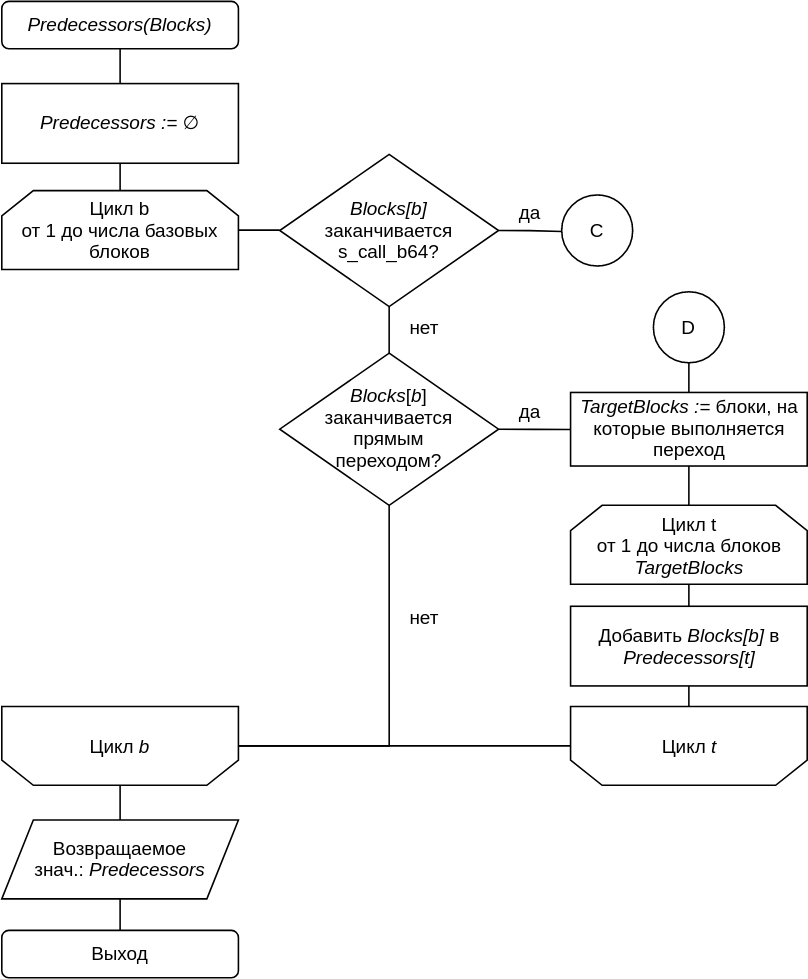
\includegraphics[width=0.75\textwidth]{diagrams/alg-cfg}
\caption{Блок-схема основного цикла опеределения предшественников}
\label{fig:diagram-cfg}
\end{figure}

Отдельно рассмотрим порядок обработки вызовов функций, обозначенный на схеме
соединителями $C$ и $D$. При условии, что пара регистров $RetGprs$, в которую
записывается адрес возврата, не изменяется при выполнении функции,
базовые блоки, из которых просходит возврат, можно определить статически.
Для этого необходимо отследить поток исполнения начиная с начала функции —
т.е. следовать по каждому прямому переходу до достижения возврата из функции
(\verb|s_setpc_b64|). Подробная схема алгоритма представлена на
на рисунке~\ref{fig:diagram-cfg-call}.

\begin{figure}[H]
\centering
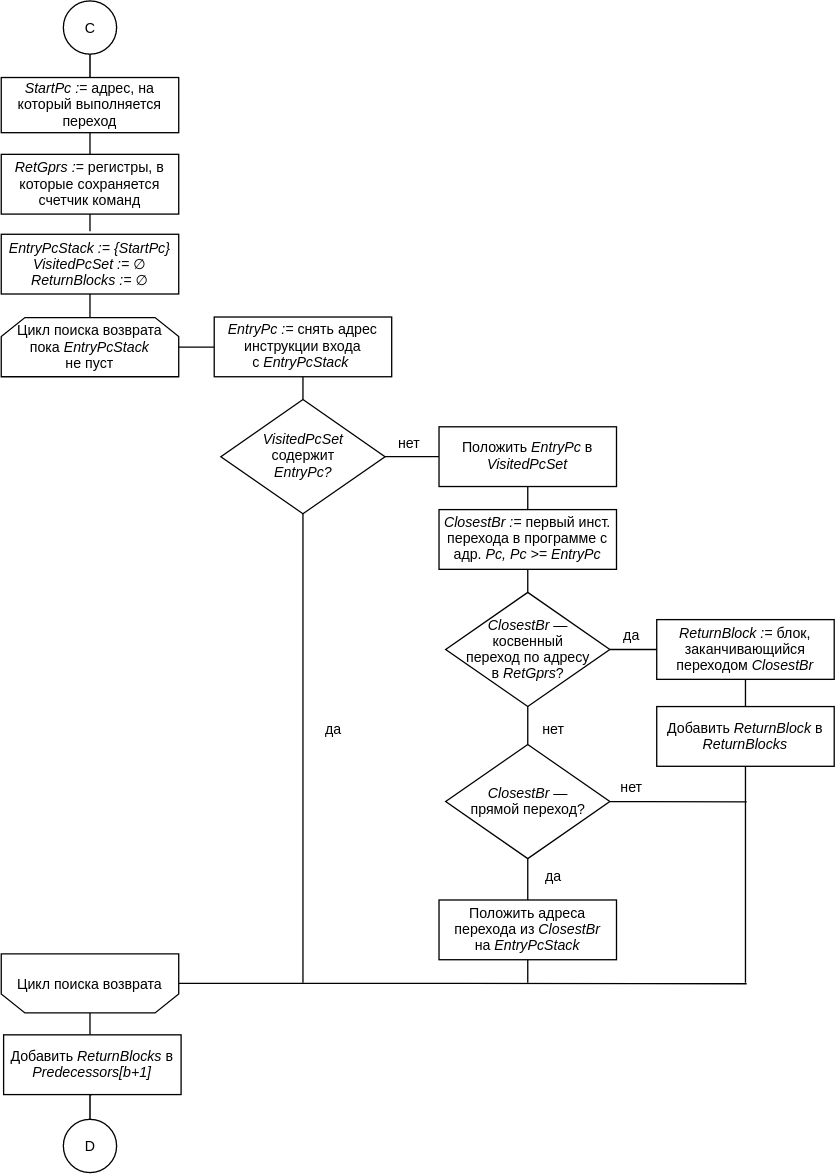
\includegraphics[width=0.8\textwidth]{diagrams/alg-cfg-call}
\caption{Блок-схема опеределения предшественников при вызове функции}
\label{fig:diagram-cfg-call}
\end{figure}

Как видно из приведенной схемы, нахождение предшественников отдельной вершины
требует анализа всех остальных вершин графа, поэтому эта задача выполняется
на этапе восстановления потока управления.

Преемники вершины, в свою очередь, могут быть найдены во время обхода графа:
на каждой итерации достаточно вычислить адреса перехода из последней инструкции в текущем блоке.
Если инструкция является вызовом функции, то адрес возврата сохраняется, затем восстанавливается
при нахождении инструкции косвенного перехода (возврата из функции).

\subsubsection{Проверка инструкций ожидания запросов к памяти}

В ходе изучения подходов к статическому анализу было установлено, что верификация
вставки инструкций ожидания является проблемой анализа прямого потока данных.
При разработке алгоритма был выбран итеративный подход, аналогично реализации,
используемой в LLVM, рассмотренной в разделе~\ref{section:gcn-waitcnt-llvm}.

В отличие от реализации, используемой в LLVM, алгоритм сохраняет состояние всей очереди
незавершенных обращений. Для каждого из обращений хранится адрес инструкции, которая его
совершает, множество затрагиваемых регистров и тип запроса.

На рисунке~\ref{fig:diagram-waitcnt} приведена блок-схема основного цикла
алгоритма, который отвечает за обход управляющего графа. Для упрощения реализации
вместо RPO-обхода базовых блоков используется прямой обход в глубину.

На рабочий стек (\textit{WorkStack}) помещается базовый блок вместе с состоянием
очереди запросов к памяти на момент входа в него. На основании этой информации
процедурой \textit{AnalyzeInstructions} находится очередь запросов на момент
выхода из блока, которая становится входным состоянием для его преемников.

Помимо этого, каждый блок \textit{BB} ассоциируется с множеством выходных состояний,
для которых был совершен обход преемников (\textit{Visited[BB]}). Если текущее выходное
состояние уже было <<посещено>>, то обход преемников не выполняется.

Однако в случае, когда базовые блоки образуют цикл, содержащий обращения к памяти без ожиданий
готовности данных, рост очереди обращений не ограничен. Чтобы гарантировать конечность
алгоритма, перед добавлением текущего выходного состояния в \textit{Visited[BB]} из него
удаляются дубликаты — обращения, исходящие из одного и того же адреса в программе. Таким образом,
множество выходных состояний монотонно увеличивается и ограничено числом обращений к памяти
во всей программе.

\begin{figure}[H]
\centering
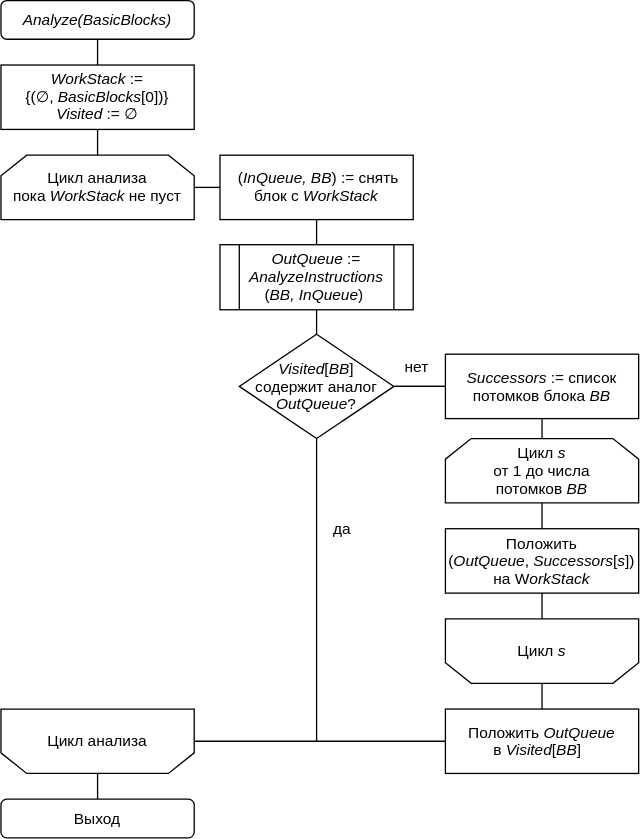
\includegraphics[width=0.8\textwidth]{diagrams/alg-waitcnt}
\caption{Блок-схема основного цикла проверки инструкций ожидания}
\label{fig:diagram-waitcnt}
\end{figure}

Рассмотрим подробнее работу процедуры \textit{AnalyzeInstructions}, блок-схема которой приведена
на рисунке~\ref{fig:diagram-waitcnt-analyze}. Она отвечает не только за нахождение нового состояния
очереди запросов к памяти, но и запись сообщений о найденных нарушениях — использовании результатов
обращений к памяти без соответвующего ожидания.

\begin{figure}[H]
\centering
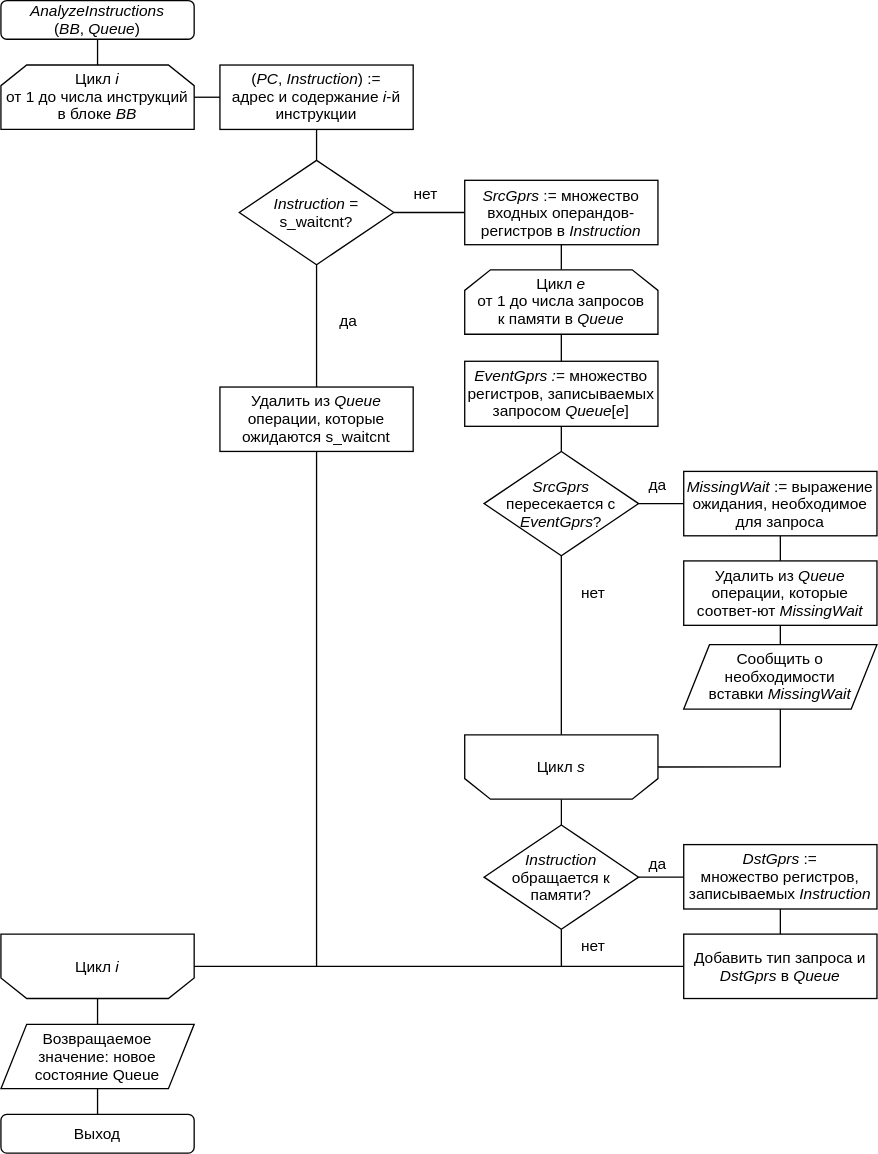
\includegraphics[width=\textwidth]{diagrams/alg-waitcnt-analyze}
\caption{Блок-схема анализа инструкций ожидания в отдельном блоке}
\label{fig:diagram-waitcnt-analyze}
\end{figure}

Основной анализа выступает цикл, который проходит по всем инструкциям в блоке. Действие, совершаемое
на каждой итерации, зависит от типа рассматриваемой инструкции:

\begin{ul}
\item Инструкции ожидания счетчиков \texttt{s\_waitcnt}: из очереди удаляются
  запросы согласно выражению ожидания (см. раздел~\ref{section:gcn-waitcnt}).
\item Инструкции, содержащие регистровые операнды: для каждого из незавершенных запросов
  в очереди проверяется, есть ли среди регистровых операндов в инструкции те,
  которые записываются данным запросом. При обнаружении нарушения информация о нем
  сохраняется для дальнейшего вывода пользователю, а в запросе очищается множество
  регистров. Таким образом, на один запрос в очереди созадется не больше одного сообщения
  о нарушении, при этом состояние очереди (число запросов) остается правильным.
\item Инструкции, выполняющие обращение к памяти: в очередь помещается информация о
  типе обращения, множестве записываемых регистров, адресе текущей инструкции.
\end{ul}

\subsubsection{Проверка слотов задержки между зависимыми инструкциями}

\todo{...}

\section{Создание программной реализации средства статического анализа}

При проектировании архитектуры и выборе платформы для программной реализации
учитывались следующие особенности описанного подхода к статическому анализу:
\begin{ul}
\item Результат анализа однозначно определяется входным значением —
исполняемым файлом. Необходимость интерактивного ввода во время работы отсутствует.
\item Процесс анализа можно представить конвейером данных, состоящим из
последовательных этапов \textit{чтения исполняемого файла}, \textit{дизассемблирования},
\textit{восстановления управляющего графа}, \textit{непосредственно анализа}.
Выходные данные предыдущего этапа являются входными данными последующего этапа.
\end{ul}

Было принято решение использовать функциональный язык программирования Haskell,
позволяющий кратко и точно описать последовательность этапов анализа
путем составления и компоновки детерминированных (ссылочно прозрачных) функций.
Полученный код легко тестировать — достаточно составить пары входных и выходных
значений для каждого модуля. Компиляция программы в машинный код сокращает время
исполнения в десятки раз по сравнению с интерпретируемыми динамически типизированными
языками программирования\cite{rwhaskell}, такими как Python.
Это отражается на применимости системы в реальных задачах разработки —
чем больше времени занимает автоматический анализ шейдеров, тем реже он будет выполняться
программистом.

\subsection{Проектирование архитектуры системы}

На рисунке~\ref{fig:diagram-arch} представлена диаграмма потока данных,
которая отражает основные компоненты системы, входные и выходные значения,
а также промежуточные артефакты.
%Пунктирной линией на схеме выделены 

\begin{figure}[H]
\centering
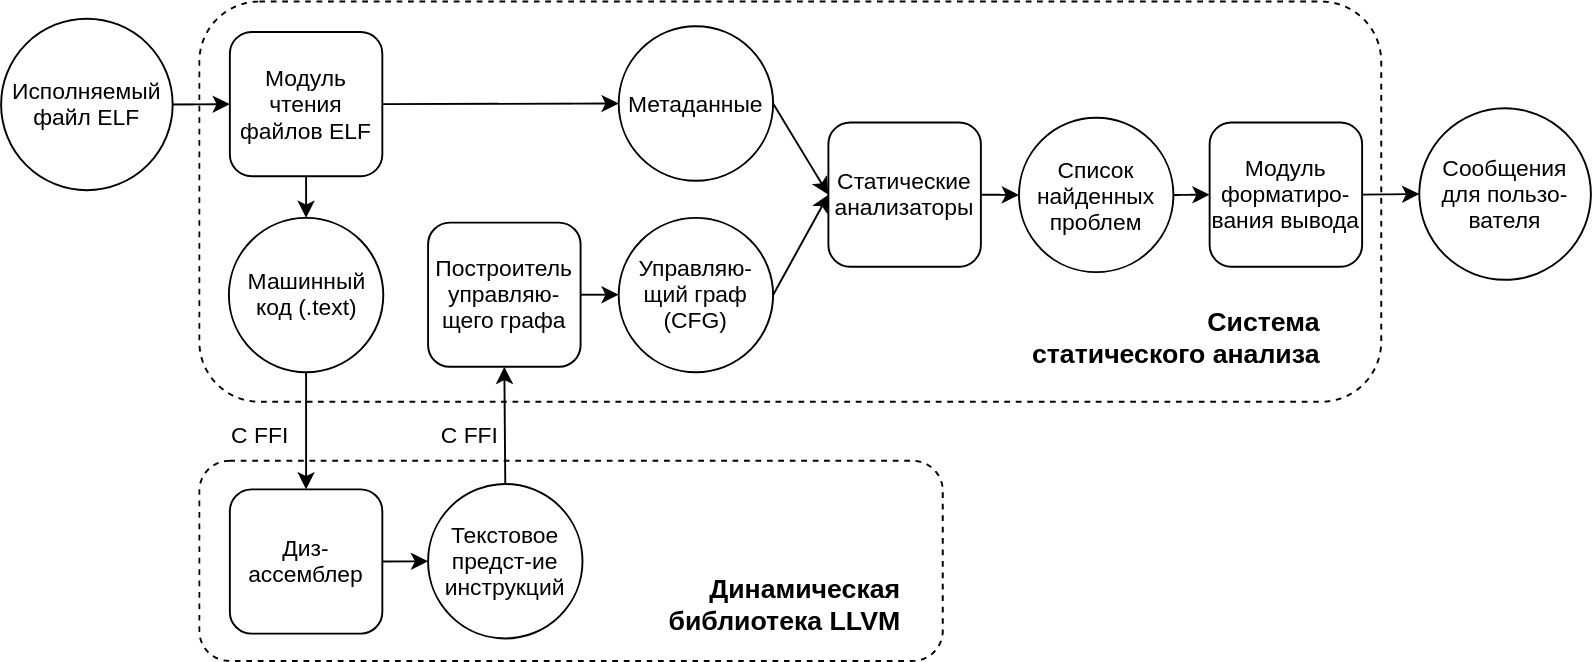
\includegraphics[width=1.01\textwidth]{diagrams/arch}
\caption{Диаграмма потока данных в разрабатываемой системе}
\label{fig:diagram-arch}
\end{figure}

\todo{...}

\subsection{Интеграция модуля дизассемблера из динамической библиотеки LLVM}
\label{section:impl-disasm}

\topic{Интерфейс прикладного программирования LLVM} Доступ к различным модулям LLVM
осуществляется через библиотеку LLVM-C. Использование дизассемблера осуществляется
в следущем порядке:
\begin{ol}
\item Инициализируется внутреннее состояние LLVM путем последовательного
вызова функций:
  \begin{inlineol}
  \item \verb|LLVMInitialize{TargetName}TargetInfo()|
  \item \verb|LLVMInitialize{TargetName}TargetMC()|
  \item \verb|LLVMInitialize{TargetName}Disassembler()|
  \end{inlineol}
Вместо \verb|{TargetName}| подставляется название бэкэнда, дизассемблер которого
используется — в нашем случае \verb|AMDGPU|.

\item Создается контекст дизассемблера для конкретного семейства процессоров
путем вызова функции \verb|LLVMCreateDisasmCPU| со следующими аргументами:
  \begin{inlineol}
  \item \verb|const char* Triple|: строка, идентифицирующая архитектуру и платформу.
Исполняемым файлам для ГП AMD на платформе ROCm соответсвует обозначение \verb|amdgcn--amdhsa|.
  \item \verb|const char* CPU|: строка, идентифицирующая семейство процессоров.
Ускорителю вычислений \textit{AMD Instinct MI100} соответствует обозначение \verb|gfx908|.
  \item \verb|void* DisInfo|: опциональный параметр для использования информации из таблицы
символов при дизассемблировании. В нашем случае не используется и выставляется в \verb|NULL|.
  \item \verb|int TagType|: опциональный параметр, см. выше. Выставляется в \verb|0|.
  \item \verb|LLVMOpInfoCallback GetOpInfo|: опциональный параметр, см. выше. Выставляется в \verb|NULL|.
  \item \verb|LLVMSymbolLookupCallback SymbolLookUp|: опциональный параметр, см. выше. Выставляется в \verb|NULL|. 
  \end{inlineol}

\item Производится считывание инструкций путем вызова функции
\verb|LLVMDisasmInstruction| со следующими аргументами:
  \begin{inlineol}
  \item \verb|LLVMDisasmContextRef DC|: непрозрачный указатель на контекст дизассемблера,
полученный на предыдущем этапе.
  \item \verb|uint8_t* Bytes|: указатель на начало области памяти с машинным кодом шейдера.
  \item \verb|uint64_t BytesSize|: размер области с машинным кодом шейдера.
  \item \verb|uint64_t PC|: смещение считываемой инструкции относительно начала шейдера.
  \item \verb|char* OutString|: указатель на область памяти, в которую будет записано
текстовое представление инструкции.
  \item \verb|size_t OutStringSize|: размер области памяти для записи текстового представления инструкции.
  \end{inlineol}
Функция возвращает число байт в считанной инструкции, то есть для дизассемблирования всего шейдера необходим цикл,
в котором к переменной $\var{PC}=0$ прибавляется возвращаемое значение \verb|LLVMDisasmInstruction| до
достижения конца программы.
Стоит учитывать, что возвращаемое значение равно нулю, если инструкция не распознана. Отсутсвие проверки
может привести к бесконечному циклу.

\item По завершении дизассемблирования ресурсы LLVM освобождаются из памяти вызовом
функции \verb|LLVMDisasmDispose|, которая принимает в качестве аргумента
непрозрачный указатель на контекст дизассемблера.
\end{ol}

\topic{Взаимодействие с подключаемыми библиотеками в Haskell} Привязка к функциям,
вызываемым из внешних библиотек, реализуется специальным языковым расширением
\cite[Глава~17]{rwhaskell}, которое включается директивой
\verb|{-# LANGUAGE ForeignFunctionInterface #-}|.

Рассмотрим декларацию одной из функций ининциализации внутреннего состояния LLVM:
\begin{verbatim}
foreign import ccall
  "llvm-c/Target.h LLVMInitializeAMDGPUTargetInfo"
  llvmInitializeAMDGPUTargetInfo :: IO ()
\end{verbatim}

В конструкции \verb|foreign import| указывается соглашение о вызовах, которое будет
использовано для обращения к внешней функции — \verb|ccall| соответствует соглашению языка С.
Затем задается заголовочный файл, содержащий сигнатуру внешней функции, и ее название.
Наконец объявляется имя функции на языке Haskell, типы ее аргументов и результата.
В приведенном примере тип функции указан как \verb|IO ()|, приблизительно соответствующий
\verb|void| в C. Это означает, что функция не принимает аргументов и не возвращает результат,
но имеет побочные эффекты — изменяет глобальное состояние.
Монада \verb|IO| гаранирует, что оптимизации компилятора не затронут порядок вызова функции
относительно других действий с побочными эффектами\cite[Глава~7]{rwhaskell}.\\

Перейдем к инициализации контекста дизассемблера:
\begin{verbatim}
foreign import ccall
  "llvm-c/Disassembler.h LLVMCreateDisasmCPU"
  llvmCreateDisasmCPU :: CString -> CString ->
    Ptr () -> CInt -> Ptr () -> Ptr () -> IO (Ptr ())
\end{verbatim}

Поскольку в Haskell используется автоматическое управление памятью,
ручное отслеживание времени жизни внешних ресурсов
может привести к утечкам памяти или ошибкам \textit{use-after-free}.
Сборщик мусора может автоматически освободить внешний ресурс, если он
обернут в тип \verb|ForeignPtr|, который также хранит указатель на функцию
освобождения. Для получения указателя на функцию перед ее именем ставится символ \verb|&|:
\begin{verbatim}
foreign import ccall
  "llvm-c/Disassembler.h &LLVMDisasmDispose"
  llvmDisasmDispose :: FunPtr (Ptr () -> IO ())
\end{verbatim}

Объявим функцию создания контекста дизассемблера, которая скрывает детали
реализации (преобразование типов для передачи в C, управление памятью, инициализацию
глобального состояния):
\begin{verbatim}
type LLVMDisasmContextRef = ForeignPtr ()

createCtx :: String -> String -> IO LLVMDisasmContextRef
createCtx llvmTriple llvmCpu = do
  llvmInitializeAMDGPUTargetInfo
  llvmInitializeAMDGPUTargetMC
  llvmInitializeAMDGPUDisassembler
  withCString llvmTriple $ \tripleStr ->
    withCString llvmCpu $ \cpuStr -> do
      ctxRefRaw <- llvmCreateDisasmCPU tripleStr cpuStr
        nullPtr 0 nullPtr nullPtr
      newForeignPtr llvmDisasmDispose ctxRefRaw
\end{verbatim}

Если примитивные значения (\verb|Int|) могут быть автоматически переведены
в соответствующие типы C, то со строками такое преобразование невозможно.
Тип \verb|char*| в C является указателем на область памяти, которая содержит символы
строки и заканчивается нулевым байтом. Стандартный тип \verb|String| в Haskell,
в свою очередь, реализован как связный список символов. Для передачи строк
используется функция \verb|withCString|, которая выделяет новую область в памяти,
копирует в нее элементы списка и добавляет нулевой байт. Указатель передается
в лямбда-выражение, которое совершает \verb|IO| действие со строкой. По завершении
действия временная копия строки удаляется из памяти.


\newpage
\phantomsection
\addcontentsline{toc}{section}{СПИСОК ИСТОЧНИКОВ}
\selectlanguage{russian}
\printbibliography[title={СПИСОК ИСТОЧНИКОВ}]

\end{document}
